\chapter{Design}
\label{ch:design}

\section{Packet capture}
\label{sec:packet_capture}

For the framework to adapt to the network environment, it must be able to listen to the network traffic.
I concluded that one of two options would be best suited to my needs:
\begin{itemize}
    \item libpcap
    \item A raw socket
\end{itemize}

\subsection{raw sockets}

Raw sockets provide direct access to low-level protocols, allowing a program to read packets down to layer two, generally the Ethernet header. 

This approach is standalone; it does not require external libraries to operate, so the program would not need pre-existing libraries installed on the system. This is particularly important in some of the applications of covert channels.

There is very little code complexity involved in setting up a raw socket:

\begin{listing}
    \vspace{0.5cm}
    \begin{minted}{julia}
# Capture the entire packet (AF -> Address Family)
const AF_PACKET = Cint(17) 
# Raw listening socket
const SOCK_RAW = Cint(3)
# Capture all ethernet frames
const ETH_P_ALL = Cint(0x0300)

socket = fdio(ccall(:socket,
    Cint, # Return type
    (Cint, Cint, Cint), # Argument types
    AF_PACKET, SOCK_RAW, ETH_P_ALL # Arguments
))
packet = read(socket)
    \end{minted}
    \caption{Raw socket listener implementation}
    \label{lst:raw_sock}
\end{listing}

Julia will read the socket pipe until an EOF is found, which marks the end of a packet; this lightweight and simplistic implementation means the construction of this listener is incredibly cheap, and thus it is very versatile.

\subsection{libpcap}

libpcap is a cross-platform library for low-level network monitoring \cite{libpcap}. 
There are a number of benefits to using libpcap, the first being the ease of implementation, libpcap provides a simple API for capturing packets, allowing for a callback function to be called when a packet is captured, this function is passed the capture header, packet pointer, and user data if required.

Because of julia's ability to integrate seamlessly with C and its libraries, the callback function could be written in julia, removing the need to write any C code. The benefit of using a library is that it is appropriately optimised. libpcap creates a memory-mapped ring buffer for asynchronous packet reception [PACKET\_RX\_RING - https://man7.org/linux/man-pages/man7/packet.7.html], this allows the userspace to the packet data without the need for need for system calls, and the shared buffer also reduces the number of copies required.

While the platform-independent nature of libpcap is beneficial, the scope of this project is limited to linux, and thus this will not be included in my evaluation.

\subsection{Conclusion}

Both raw sockets and libpcap are viable options for packet capture, however, libpcap has a few advantages, the factor that swayed my decision was the support for the Berkeley Packet Filter (BPF). BPF's are register-based "filter machines" [The BSD Packet Filter] that makes filtering packets incredibly efficient, this is particularly useful for this project as it allows for the filtering of packets to be done in the kernel, which reduces the number of packets that need to be processed by the program. Specifically, this means the receiver can filter traffic so it only has to process packets that are destined for it, reducing the overhead.

\subsection{Note}

Eventually I decided that both implementations could be used in the framework, the raw socket was used to capture packets for the sender, without disrupting the main queue of packets. The additional code complexity of searching the queue did not outweigh the overhead of opening a raw socket, there are also some other benefits to using the raw socket, but I will discuss them in context in \ref{sec:integrity_impl}.

\section{Packet processing}

\dots

\section{The Queue}
\label{sec:queue}

The queue is essential to the operation of the framework, it is how the packets are put by the listening thread, and retrieved by the main thread for processing.

Initially, I was using a \inline{Channel} data structure, it is a thread-safe, waitable, First-in-First-out queue [JULIADOCS] that worked for the most part, however it introduced a bug into my codebase that meant the listening thread would block the main thread while it was waiting for packets, thus the covert channel would not run in a silent environment.

While this isn't a huge problem, since a covert channel is quite exposed on a silent network, it is not ideal. I eventually decuded that I was improperly accessing the properties of the structure, I was attempting to get the whole queue without removing the items, so I just took it from the underlying array. Unfortunately, the \inline{Channel} is locked by default, and thus the main thread was being blocked until the listening thread pushed something to the queue.

While I knew this action was not truely thread-safe, meaning I would likely be operating with stale data, it wasn't of great importance that my queue was truely up-to-date, as I was taking a rolling average of 150 packets anyway. I didn't realise that it would cause the main thread to be intermitently blocked, additionally, this unusual behaviour meant that it was difficult to debug, especially since my print statements were reliant on packets being received by the listening thread, which caused a lot of debugging cycles to be performed.

My solution to this was to implement a new, more idomatic datastructure, the \inline{CircularChannel}. This is a thread-safe, waitable, First-in-First-out queue that behaves like a circular buffer, so that it overwrites the oldest item when it is full.

\begin{figure}[!h]
    \begin{minipage}{0.5\textwidth}
        \centering
        \begin{minted}{julia}

packet = get_packet()
if isfull(queue)
    take!(queue)
end
put!(queue, packet)

        \end{minted}
        \captionof{listing}{Old "Channel" implementation}
    \end{minipage}
    \begin{minipage}{0.5\textwidth}
        \centering
        \begin{minted}{julia}

packet = get_packet()
put!(queue, packet)

        \end{minted}
    \captionof{listing}{New "CircularChannel" implementation}
    \end{minipage}
\label{lst:queue_comparison}
\end{figure}

By overloading the \inline{put!} and \inline{take!} functions, I was able to implement their functionality for my new data structure, this meant for most of the code all I had to do was replace the type annotations of \inline{Channel} with \inline{CircularChannel}. This is ofcourse with the exception of the queue, whose changes can be see in \ref{lst:queue_comparison}, and the \inline{get\_queue\_data} function that I was using to improperly access the queue, thanks to my use of a central function for accessing this queue data I was able to change the implementation of the function without having to change the code that called it. I did this by creating a type convert funtion for the \inline{CircularChannel\{T\}} to \inline{Vector\{T\}}, where T is any data type, since I implemented this in a thread-safe way, I was able to use altered \inline{get\_queue\_data} function to access the queue data without blocking the main thread.

I efficiently achieved this waiting using \inline{Conditions}, they are locks that implement \inline{wait} and \inline{notify} methods that block (reducing resource usage) and release threads, respectively, based on the status of the condition. This allows my main thread to wait for the listening thread to push a packet to the queue, and then continue processing the packet (for the receiver only).

\subsection{Queriability}

One of my goals for the project was to allow any type of covert channel to be used in the framework, regardless of classification. Ultimately, this meant I was going to have to take a dynamic approach to the initialising and using channels. I concluded that it was best to be able to query the channel for certain properties in packets, like the destination port or the packet size.

I implemented a rudimentary query system, that allowed for querying of properties captured by the framework (known header values), these properties could be combined with simple logical operators (AND, OR) to sufficiently complex queries. An extract of Faucet's documentation gives an example of what these queries look like:

[ADD DOC EXAMPLE]

\section{The target (Arrangemnt)}
\label{sec:target}

Covert communication is reliant on a preshared arrangement \cite{DoCCaS}, this arrangement is a set of parameters that both parties will assume the other is using, it contains the following information:

\begin{itemize}
    \item The IP Address of the target.
    \item The covert methods to use.
    \item The AES Pre-shared key.
    \item The Initial Vector to use.
\end{itemize}

The IP address is where the sender will send the packets, and the address the receiver will listen on. In theory, this address does not have to be the address of the target, as long as the target can see that endpoint, but I cannot test this due to limitations in the testing environment. The covert methods are the channels that will be used for communication, they are referenced by their index in the array of covert methods, and thus the order of the covert methods is important.
The AES pre-shared key is used to encrypt (and subsequently decrypt) the data, and the initial vector is used to initialise the AES encryption.

\section{Sending packets}
\label{sec:sending_packets}

Sending packets is an important aspect of the framework, as outgoing packets must be completely composable to permit all covert channels. While Julia does have some socket functionality, it is not sufficient for the project as it is too high level, my implementation instead uses a lightweight TCP/IP stack design. The principle is the user can supply the protocols to use, and a dictionary of fields and values for each of the layers, The function will then construct the packet, filling in an informed manner.

For example, in an IP header, source and destination fields will default to the local ip and targets ip respectively, But in a TCP Header, the ISN will be random. If flags are set, but their respective fields are not filled, they will also randomised. This allows for the user to specify the fields they want to be set, and the rest will be filled in a way that is consistent with the protocol, however it should be noted that some of these randomised fields do not have uniform distributions, and thus may be more suspicious than others, but this is out of the scope of my project.
 
Since thes filling of these additional fields is done at execution time, a "skeleton" packet can be created that outlines a basic packet, then this skeleton can be used multiple times without having random fields being static, it is also useful with packet checksums, as this burden is not passed to the user. I make use of this functionality in the used of covert modules, as outlined in \fullref{sec:covert_modules}.

The packets themselves are sent over a raw socket, this allows for the packet to be sent without the kernel imposing checks on its validity (such as the checksum), this is important for the operation of some covert channels, as they create packets that would otherwise be dropped by the kernel (sometimes because of firewalls). For a packet to be sent over a raw socket at the link layer (ethernet) it needs to be sent with a \inline{sockaddr\_ll} struct, outlined in [man Packet(7)] the majority of these fields are not required, or are unlikely to change (The physical layer protocol) and thus can be hardcoded, only two fields need to be created populated dynamically, the interface index and the destination mac address. The interface used is the one that the queue listens on, and the destination mac can be taken from the packet.

The packets can then be sent to the raw socket using the \inline{sendto} function, taking the socket, packet and \inline{sockaddr\_ll} as arguments.

\section{Providing context to the sender}
\label{sec:context}

Many of the senders functions are reliant on the context of the environment, this environment is constructed as a dictionary of values that are passed to the sender. This dictionary contains the following values:

\begin{itemize}
    \item The desired secrecy of the channel (User argument).
    \item The interface to use (see \fullref{sec:sending_packets})
    \item The socket to send packets over.
    \item Information about the route to the target.
    \item The queue
\end{itemize}

I will discuss the desired secrecy argument in \fullref{sec:decision_algorithm}, and the interface has already been discussed in the construction of the \inline{sockaddr\_ll} struct (see \fullref{sec:sending_packets}). The socket is simply a raw socket, in does not carry context and thus could be recreated at each use, but that requires calls to the kernel, and this approach has very little overhead.

The information about the target essentially outlines the default path to follow for a target, like the physical address of the target, or the gateway to use to reach the target. while this is not applicable to all channels, it is used for many of them, and not worth recalculation for each packet.

The queue is also exposed here, since it accounts for most of the context of the sender, compiling these contextual values into a single dictionary makes it easier to pass around, and allows for the sender to be more idomatic.

\section{Design of covert modules}
\label{sec:covert_modules}

A covert module is a set of functions that are used to implement a covert channel. For the framework to work effectively, the addition of covert modules must be a process that is both simple and idomatic, but sufficiently flexible to allow for any type of covert channel to be implemented. Since I cannot predict the nature (and thus the requirements) of the covert channels that will be implemented, A dynamic approach is required.

Covert modules are implemented using:
\begin{itemize}
    \item An \inline{init} function.
    \item An \inline{encode} function.
    \item An \inline{decode} function.
    \item A \inline{covert\_method} struct instance.
\end{itemize}

The \inline{init} method is called when the module is loaded, it is used to initialise the channel, and it returns a set of keyword arguments that are to be passed to the \inline{encode} functions, the most common of these arguments will be \inline{template}, which outlines the skeleton and structure of a packet that the covert channel lives in, omitting the fields that are to be used in the channel, as outlined in \fullref{sec:sending_packets}. This function is passed the queue (see \nameref{sec:queue}) to allow it to adapt to the environment.

Covert channels can be adapted to the network on a sub-method level to improve covertness, a good example of this is using IPv4 vs IPv6 as the internet protocol, for covert channels that exist all other layers this does not affect their operation, but does allow them to be better suited to the network. I Specifically chose to implement the TCP Acknowledgement bounce covert channel to showcase this flexibility in the framework, By using a local TCP server to bounce the packets, the channel must be aware of the network to discover these hosts. For this to be possible, the \inline{init} function must have the environment exposed to it, this is done by passing the environment dictionary outlined in \ref{sec:context} to the \inline{init} function.

In the case of the TCP Acknowledgement bounce covert channel, the queue is taken from the environment dictionary, and the \inline{init} function will use this to listen for the destination of TCP packets, and it will return a template that has the destination mac, ip and port set to the local server.

The \inline{encode} function is called for each packet to be encoded, it is passed the keywords arguments from \inline{init} and the payload to put into the packet. The function will then return a full packet template, that can be converted into a vector of bytes, and sent over the network.

The \inline{decode} function is called to extract the payload from a packet, it doesn't require any other arguments as it just returns the field of the packet object that has the payload in it. This function does not need to perform any validity check, as the framework will verify that the packet could contain the payload before calling this function.

The \inline{covert\_method} struct holds metadata about a channel, and is comprised of five fields:
\begin{itemize}
    \item The name of the covert channel.
    \item The TCP/IP layer it operates on.
    \item The protocol in that layer it operates on.
    \item How covert it is, on a scale of 1 - 10.
    \item The bit capacity of the channel.
\end{itemize}
\label{itm:covert_method}

These allow the framework to seamlessly integrate with the covert channel, for example the bit capacity is used crafting payloads for the channel, removing this burden from the module. The name of the channel is used in \fullref{sec:target} to ensure both parties are using the same cha

The layer and protocol are used by the receiver side of the framework to filter out packets that are not relevant to the covert channel, so the \inline{decode} function is only called on packets that are valid, so error handling can be omitted from covert modules, unless they are particularly complex.

All of the fields are used to creating an informed decision on which covert channel to use, as outlined in \fullref{sec:decision_algorithm}.

\subsection{Covert module validation}

Covert modules need to be validated before they can be used in the framework, this is done to ensure they are compatible with the preshared arrangement (defined in \fullref{sec:target}), there are three checks to be performed:

\begin{itemize}
    \item The smallest channel is not smaller than the minimum channel size.
    \item The number of channels is not too large to be represented by the minimum channel size.
    \item The channels are in the same order they appear in the arrangement in.
\end{itemize}

The first check prevents very small channels being used in the framework, as they are not large enough to carry the \fullref{sec:microprotocols}. The second check prevents too many channels being used, as the micro protocols need to be able to uniquely identify each one, if there too many channels then they cannot be used (but since they have been registered they can still be considered when picking an algorithm, causing an failure in the communication).

Since the channels are referenced by their index, both the sender and receiver need to be using the same channels, in the same order, this is why the third check is required.

\section{Decision algorithm}
\label{sec:decision_algorithm}

The decision algorithm is responsible for the adaptive nature of the framework, it is used to decide which covert channel is best suited to the current environment.
The algorithm is an empirically derived function that takes the following arguments:

\begin{itemize}
    \item $E_s$ - The desired secrecy of the environment
    \item $L$ - An array of dictionaries, describing the protocol usages in the environment
    \item $E_r$ - The rate of packets in the environment
    \item $E_h$ - The number of active hosts in the environment
    \item The covert methods to choose from.
    \item Penalised methods.
    \item Index of the current method.
\end{itemize}

While $E_s$ is a user argument, $L$, $E_r$, and $E_h$ are derived from \fullref{sec:queue}. Penalised methods have a penalty on their score, to discourage the algorithm from picking them again, why these methods are penalised is discussed in \fullref{sec:penalising}, and the index of the current method is used to discourage the constant switching of channels.

The output of this algorithm is two arrays, $R$ and $S$ where $R_i$ is the rate of the $i^{th}$ covert channel, and $S_i$ is the score of the $i^{th}$ covert channel.

For a deeper understanding of the algorithm, see \fullref{sec:algorithm_impl}.

\subsection{Covertness}

$C_i$ is the covertness of the $i^{th}$ covert method, it is calculated using the covertness of the channel defined in \fullref{itm:covert_method}, and the desired secrecy of the environment, a user argument. The covertness of the method is correlated to the desired secrecy of the environment, and thus it is not just the covertness of the channel.

This way, methods that are more covert than the desired are given a score boost, and methods that are less covert than the desired are penalised.

The covertness of the channel is calculated using the following equation:

\begin{equation}
    C_i = 1 - \frac{E_s - M_c}{10}
\end{equation}

Where $M_c$ is the covertness of the channel, and $E_s$ is the desired secrecy of the environment.

If the desired secrecy was 5, and the channel had a covertness of 3, $C_i$ would be 1.2 (a 20\% boost to the score). Conversely, if the desired secrecy was 10 and the channel had a covertness of 3, $C_i$ would be -0.7 (a 70\% penalty to the score).

The reason to not just prevent the use of more covert channels is because the covertness of the channel is also correlated to its use in the environment, if a covertext is very prominent in the environment, the covertness of the method will be higher and thus a better choice than a slighty more covert, but less common method.

$C_i$ is within the interval $[0.1, 1.9]$ (-90\% to 90\% penalty/boost).

\subsection{Rate calculation}

The rate of a channel determines how often packets should be sent over that channel while remaining covert. This is a function of the rate of packets in the environment, the number of active hosts in the environment, and the covertness of the channel.

The rate of the channel is calculated using the following equation:

\begin{equation}
    R_i = \frac{E_h}{P_i * E_r * \frac{C_i}{2} }
\end{equation}

Where $P_i$ is the percentage of packets in the environment that use the protocol of the $i^{th}$ channel, and $E_r$, $E_h$ and $C_i$ are as defined above. The reason for the $\frac{C_i}{2}$ term is to prevent the rate being higher than estimated protocol output per host per second ($\frac{E_h}{P_i * E_r}$) as this would cause the channel be using a protocol more than the average host, and thus be more suspicious.

$R_i$ is within the interval $[0, \infty)$.

\subsection{Score calculation}

The score of a method is a function of its use in the environment, its capacity, and its covertness.
The score is calculated using the following equation:

\begin{equation}
    S_i = P_i * B_i * C_i
\end{equation}

Where $P_i$ is the percentage of packets in the environment that use the protocol of the $i^{th}$ channel, and $B_i$ is the bit capacity of that channel. $C_i$ is as defined above.

The $P_i * B_i$ term is the effective bandwidth of the channel, we'd like out covert communication to be as fast as possible, and thus the higher the effective bandwidth, the better. We again factor in the relative covertness ($C_i$) of the channel to the desired secrecy.

\subsection{Preventing constant switching}

The index of the current method is used to prevent the constant switching of channels, this is done by giving a bonus of 10\% to its score, this percentage is arbitrary, but it is large enough to work, and small enough to allow for the channel to be switched if it is not covert enough.

For a method a method to be chosen, it must be more than \%10 better than the current channel, if it exceeds this threshold it will be chosen, and will gain a +10\% bonus to its score, and the previous channel will lose its bonus, effectively putting a \%20 gap between them. This encourages the channel not to change again, unless it is significantly better than the current channel.

\section{Microprotocols}
\label{sec:microprotocols}

The adaptive covert channel is reliant on the underlying protocols, these protocols are used to implement:
\begin{itemize}
    \item Describing the nature of a payload
    \item Starting communication
    \item Ending communication
    \item Switching active channel (The one being used for communication)
    \item Verifying integrity of the communication
    \item Discarding chunks of data that have been corrupted
    \item Recovering from a disconnection in communication
\end{itemize}
\label{itm:microprotocols}

A sentinel signal is sent to begin and end communication, this way they can both share the same microprotocol, once a sentinel is received, then the receiver starts to build the context of the communication, like the received data and the current chunk.

Data is sent in chunks, a chunk is effectively a buffer of data that has not had its integrity verified yet, once the verification of the chunk has passed, it can be commited to the main buffer, and the chunk can be emptied ready for the next set of data. Both the sender and receiver keep track of this chunk so the state of communication is atomic between the two parties.

Inorder to implement these protocls effectively, using the contextless design proposed in \fullref{sec:DRiCCBoCP}, packets need to desribe their nature, I decided to implement this using a single bit, at the start of the payload. 0 or 1 indicate whether the packet is data or metadata, respectively. Protocols are implemented as metadata, and are of adaptive length, the size of these protocols is a function of the number of underlying channels that may be used. The minimum channel size is $1 + \floor{log_2{M_c + 1}}$ where $M_c$ is the number of underlying covert methods.

For some protocols, it is beneficial to use more than the minimum channel size, for example, when verifying the integrity of a channel an offset can follow the protocol. The offset is assumed to be 0 if it is not present, but when it is present it improves the covertness of the channel, exactly why this is the case is discussed in \fullref{sec:integrity}. For the chunk discarding protocol, the space following the protocol is filled with payload data, this is because the sender will have to resend the previous data segments and without doing this there would be repeated fields, which would be suspicious to an observer.

For protocols that do not have auxillary data to be sent with them, the following data bits are assigned at random, this has no benefit to the covertness of the channel, since the payload is encrypted and thus appears random, however the added complexity of the protocol for the tradeoff of bits did not seem worth it.


\subsection{Protocol compression}

The compression technique outlined in \fullref{sec:DRiCCBoCP} is Huffman coding, which is a simple lossless compression technique that maps the protocols to a number, then the binary representation of that number can be used, however I do not think this method of compression is best suited to the framework. The problem with huffman coding arises when the distribution of protocol is not uniform, In my case the majority of traffic will be data, and thus by using only the first bit to declare it as data, the rest of them will be data. The consequence of this is the metaprotocols will be slightly larger that otherwise, but since by their nature they are less frequent that data, this is a worthwhile tradeoff.

\subsection{consequence of this approach}

Unfortunately, using a single bit to denote data means that the orignal payload is not taken in whole bytes, A packet of n bits will carry n-1 bits of data. This creates an issue when reading the payload because the bits must be read out-of-alignment. This problem is excaserbated by the unknown nature of the packets pre-communication, as some channels have higher bit capacities, along with the introduction of chunk retransmission, it is not feasible to precompute the possible payloads. The solution I found for this problem was to store the payload as a bitstring, the base two representation of the number in string form, then read the desired number of bits from the string. There is a time and space cost of storing the payload like this, and in hindsight using a \inline{BitVector} would be more performant, but this cost is negligble and the code is easier to follow than using bit shifts to read the bits.

\section{Transmission padding}

The common approach to adding bits of padding is to append the data with a 1, and fill any remaining space with 0's, the cost of this (minimum number of bits added to the payload) is 1, which is the lowest possible. While this application works well for non-covert scenarios, it can create particularly suspicious looking payloads, the worst case scenario of this is an entire packet with a single 1 followed by 0's to fill capacity.

In this paper I will propose a soluton that is better suited to covert channels, it does have a higher space cost, however the benefit is more of the data is random. The cost is logarithmically proportional to the size of the data, altough if the data has fixed size increments (a common one would be bytes as most payloads will be byte data) then the length can be divided by this number to reduce its costs. In my case, the AES encryption means that the data is a multiple of the key size (128 bits) so the equation of my cost complexity would be $log_2(l/128)$ where $l$ is the length of the encrypted data.

[HOW PADDING WORKS DIAGRAM]

The padding method works by storing the (reduced) size of the encrypted payload after the encrypted payload, and the remaining padding can almost be random. The data is read from right to left, and the sender must ensure that the first valid length is the one that describes the payload. For scenarios where the largest payload size is smaller than the smallest increment size, this is not necessary.

Both of these padding methods will be tested and compared in \fullref{sec:padding_testing}.

\section{Verifying communication integrity}
\label{sec:integrity}

Verifying the integrity of communication is essential to the operation of the framework, it allows the communication channel to remediate any errors that may occur, and thus allows for the communication to be more reliable. The integrity of the communication is calculated using an 8-bit cyclic redundancy check (CRC-8). This allows errors to be recovered from using the discard chunk protocol (outlined in \fullref{sec:microprotocols}).

This requires the receiver to be able to communicate the integrity of the message back to the sender, so the sender can decide wheter to resend the chunk or not. In-order to do this the medium of communication must be both undisruptable, and broadcasted.

The communication must be undisruptable because if the sender does not received the integrity of the message, it will assume the receiver did not receive the message, and thus resend it.

It must also be broadcastable because there is no garuntee that the receiver will be able to determine the address of the sender, this is particularly true in the case of the TCP Acknowledgement bounce covert channel, as the sender will be using a local server to bounce the packets, and thus the receiver will not know the address of the sender.

A covert channel based on the Address Resolution Protocol (ARP) (outlined in \fullref{sec:ARP}) suited both of these requirements perfectly, as it is broadcasted, and it required for the normal operation of a network, thus it is undisruptable. There are some applications where the ARP Beacon is not suitable for use:

\begin{itemize}
    \item The sender is not on the same network as the receiver.
    \item The network is solely IPv6 (using Neighbor Discovery Protocol (NDP) instead of ARP).
    \item The nodes of the network are statically configured.
\end{itemize}

Where ARP is not applicable, a different means of communication must be used, however that is out of the scope of this paper.

The verification process is a challenge and response protocol, the sender will send a challenge to the receiver, and the receiver will respond with the integrity of the message. Verification of data chunks is performed when the method change protocol is sent, this is when the communication medium changes and thus the framework seeks to verify that the previous channel was successful. This does delay the verification of the data until the start of the next method transmission, but it does mean that the verification can be can become an implicit part of the method change protocol, which keeps the minimum channel size low, and reduces the number of packets sent. This method still allows a 
challenge to be perfomed without changing the channel, by sending the method change protocol to the current channel index, this is useful for continual verification of the channel, but it does increase the number of packets sent.

To improve the covertness of the ARP Beacon, the sender will (if the channel is large enough) provide an offset to the receiver, the receiver will XOR this with the result of the integrity check. Since the sender knows the correct integrity of the data, it can find an active host on the network and XOR the integrity with the host byte, the outcome of this is an offset that the receiver can use to make its ARP request look valid to an observer. This is only possible if the channel is large enough, but if it is not the receiver will assume no offset.

With the offset the ARP Beacon is much more covert, and less prone to detection from Aware active wardens. However, this is only true when the integrity of the data is correct, if the data is corrupted, then the request will point to the wrong address, which could raise suspicion. Unfortunately, the receiver cannot determine wheter the integrity is correct without sending its response, so this is a tradeoff that must be made.

There are some addresses that are blacklisted from being used, for example, the address of the sender (as they are in communication, the receiver could send an ARP packet that is unrelated to the covert channel, which could cause issues). The broadcast and network addresses are also blacklisted, as they are not valid hosts on the network, and thus would be suspicious to an observer. 

\begin{figure}[h]
    \centering
    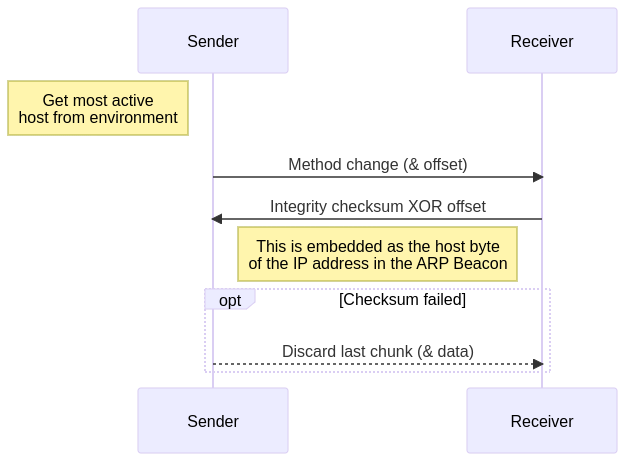
\includegraphics[width=0.8\textwidth]{fig/Integrity.png}
    \caption{Integrity challenge and response (optional parts in brackets)}
    \label{fig:integrity}
\end{figure}

Since the sender knows what the what the response is supposed to be, it can await the response and succeed quickly (if it sees the expected response), otherwise it will wait until the timeout expires (5 seconds by default). Unfortunately, the sender cannot accurately tell if the receiver has not received the packet, or if the integrity is incorrect, since the host is assumed to be using ARP communication outside of the channel.

This challenge and response process can be perfomed irrespective of the underlying covert channel, but it might require limitations on the environment (just as ARP requires a local network). 

\section{Communication failures}

There are scenarios where the channel for communication no longer works, this could be of a change in the environment, or a warden that has prevented the channel. In these secnarios the framework must be able to recover the communication effort, the sender and receiver need a sort of fallback channel that they can use to restart communication. However, if the fallback channel was the one being blocked then the communication would have to end, even if other channels were viable.

To prevent this, a recovery mode is defined for the framework, in this mode the receiver is open to all channels, and the sender will iterate through possible channels until it finds one that works. To prevent this happening unintentionally the recovery mode is only entered when:
\begin{itemize}
    \item The receiver has failed two consecutive integrity checks.
    \item The receiver has not received any covert data for an interval.
\end{itemize}

Either one of the above conditions will send the sender/receiver into recovery mode, and the other one will eventually do the same. The sender will purposely wait until the interval has passed before attempting to recover, this is to prevent the sender from trying to switch channels prior to the receiver entering the recovery mode. This interval is based on the time and packets of the last verified chunk (the number of packets between verification, and the time between verification), this interval must be exceeded by 50\% before receiver will enter recovery, and the sender will wait for even longer before attempting to recover. It is important to note that since this time between verifications could naturally exceed the interval, the receiver will still acts as if the current channel is viable, saving the data to the chunk (Although this chunk will be discarded implicitly if the channel is "recovered").

The recovery mode can be recovered with a specially crafted packet, this packet should begin with the sentinel signal (as if it was starting communication) followed by the length of verified data, and an offset. The offset is used for the same function here as it is in \fullref{sec:integrity}, however it is used in combination with the length of verified data, this is the length of the last sender verified data. There are some cases where the receiver will have assume its last verification was valid, but in reality the discard chunk failed to reach it, but the sender will always know the length of the data at the last verification.


Since this packet requires more space than the minimum channel size, there are some cases where it does not fit in a channel, in these cases it simply cannot be used, and the alternative is to recover to a method with a larger bit capacity, then switch to the higher scoring channel afterwards. While this requirement is not perfect, it is the best way to prevent receiver breaking communication due to interference from external sources.

When the receiver is recovered, it will send an integrity check back to the sender so it knows that the recovery was successful, the intervals between verifications here will not be recorded since it may not be consistent between the sender and receiver.

\subsection{Penalising methods}
\label{sec:penalising}

This recovery process is not great for covert communication, and causes the sender to try multiple channels, if these other channels are blocked then it can raise suspicions, to discourage this we penalise methods.

When a method fails twice, causing the recovery process to occur, it receives a penalty of -90\% to its score. This penalty lasts for 30 packets of valid data communication and prevents the method being chosen again unless there are no better alternatives. The reason we do not permenantly block the protocol is beacuse it can fail for reasons that are temporary, but we cannot know that until we try again, It is not a good idea to constantly retry failing methods as if they are being caught by wardens then it is much more suspicious for a many packets to have been prevent rather than just a few.
